\emph{Como producto del trabajo presentado en este capítulo surgió un proyecto de código libre alojado en Github,\footnote{\url{https://github.com/sergioburdisso/pyss3}} el cual, a la fecha, posee más de 180 estrellas y más de 35 mil descargas registradas por parte de la comunidad. Además, también surgió el artículo ``PySS3: A Python package implementing a new model for text classification with visualization tools for Explainable AI'' enviado a ``Computing in Science \& Engineering'', el cual se encuentra actualmente bajo revisión.}
% \emph{Como producto del trabajo presentado en este capítulo surgió el artículo publicado en ``Pattern Recognition Letters'', volume xxx, titulado ``$\tau$-SS3: A text classifier with dynamic n-grams for early risk detection over text streams''.}\footnote{\url{https://doi.org/10.1016/j.patrec.2020.07.001}}

% \

\section{Introducción}

% clasificador general
El clasificador de texto que hemos introducido y desarrollado en este trabajo doctoral fue especialmente diseñado para lidiar con tareas de detección anticipada de riesgos, por este motivo fue dotado con ciertas cualidades como parte de su diseño, como son su capacidad de trabajar incrementalmente, tanto para entrenar como para clasificar, y su transparencia, al tener la capacidad de explicar los motivos de la clasificación.

No obstante, no hay elementos en su diseño que lo limiten a ser utilizado exclusivamente en este tipo de tareas, ya que fue definido de forma general.
De hecho, este clasificador es en esencia un modelo de clasificación de texto de propósito general, como cualquier otro clasificador convencional ---\emph{e.g.} \ac{MNB}, \ac{SVM}, k-NN o las Redes Neuronales, entre otros.
Además, creemos que podría llegar a ser especialmente útil en aplicaciones en las que comprender las razones detrás de las predicciones del modelo ayudarían, ya sea a los usuarios, desarrolladores o investigadores, a decidir cuándo confiar o no en él.
Este último aspecto no es menor si tenemos en cuenta que cada vez más aplicaciones de aprendizaje automático piden a los usuarios que confíen en un modelo que les ayude a tomar decisiones, no sólo en aplicaciones de riesgos, sino también en situaciones de bajo riesgo, como simplemente al elegir qué producto comprar o qué película ver, se requiere cierto grado de confianza antes de ceder nuestro dinero u horas de nuestro tiempo sólo en base a un ``porque el modelo lo dice''.

Por este motivo, y dado que Python es el lenguaje de programación más popular dentro de la comunidad del aprendizaje automático gracias a su sintaxis simple y un rico ecosistema de implementaciones eficientes de código abierto de algoritmos populares~\cite{python2007}, decidimos crear un paquete Python oficial de código abierto para que cualquier interesado pueda utilizar a SS3 en la tarea de clasificación de texto que necesite, ya que creemos que la disponibilidad de implementaciones de código abierto es de vital importancia para fomentar el uso de nuevas herramientas, métodos y algoritmos.
Así, en este capítulo presentamos y compartimos a ``PySS3'', un paquete Python de código abierto que implementa SS3 y que, además, incluye un conjunto de herramientas útiles que permiten trabajar con él de una manera visual, interactiva y directa. Por ejemplo, una de estas herramientas proporciona explicaciones \emph{post-hoc} utilizando visualizaciones que resaltan directamente las partes relevantes del documento de entrada, lo que le permite a los investigadores y desarrolladores comprender mejor a sus modelos.
% In this work, we introduce ``PySS3'' and share it with the community. PySS3 is an open-source Python package that implements SS3 and comes with two useful tools that allow working with it in an effortless, interactive, and visual way. For instance, one of these tools provides post-hoc explanations using visualizations that directly highlight relevant portions of the raw input document, allowing researchers to better understand the models being deployed. Therefore, PySS3 could be especially useful for those working with sensitive classification problems by which people's lives could be affected since it allows researchers and practitioners to deploy explainable and more reliable models for text classification. 


\section{El Paquete Python PySS3}\label{sec:pyss3}

En esta sección se introduce el paquete desarrollado, en particular se comienza describiendo brevemente su arquitectura, resaltando sus principales módulos, luego se examina su funcionamiento general, y finalmente se brindan ejemplos ilustrativos de su utilización.

\subsection{Arquitectura de Software}

PySS3 se compone de un módulo principal y tres submódulos.
El módulo principal, llamado ``pyss3'', contiene la implementación del clasificador propiamente dicha por medio de una clase llamada ``SS3''.
% PySS3 is composed of one main module and three submodules. 
% The main module is called ``pyss3'' and contains the classifier's implementation \emph{per se} in a class called ``SS3.''
Esta clase no sólo brinda la implementación de la versión original del clasificador, sino también la extensión introducida en el \autoref{cap:tss3}, que le permitió al modelo reconocer n-gramas de palabras relevantes.
% The $SS3$ class implements not only the ``plain-vanilla'' version of the classifier \cite{burdisso2019} but also different variants, such as the one introduced later by the same authors \cite{burdisso2019-tss3}, which allows SS3 to recognize important word n-grams ``on the fly.''
Además, como se verá en los ejemplos de la \autoref{sec:eg-1}, esta clase también expone una \emph{API} clara y simple, muy similar a la de los modelos de \emph{scikit-learn} ---por ejemplo, incluye los conocidos métodos ``fit'' y ``predict'' para el entrenamiento y la clasificación, respectivamente.\footnote{La lista completa de los métodos brindados por esta clase se encuentran disponible en la documentación de la API:  \href{https://pyss3.rtfd.io/en/latest/api/index.html\#pyss3.SS3}{\url{https://pyss3.rtfd.io/en/latest/api/index.html\#pyss3.SS3}}}
Finalmente, este módulo principal ``pyss3'' se divide en los siguientes tres submódulos:
% Additionally, as the reader will notice in the example shown in , the $SS3$ class exposes a clear and simple API that is similar to that of \emph{Scikit-learn} models . For instance, it provides standard methods like ``fit'' and ``predict'' for  training and classification, respectively. The complete list of SS3's methods is available in the API documentation (\href{https://pyss3.rtfd.io/en/latest/api/index.html\#pyss3.SS3}{\url{https://pyss3.rtfd.io/en/latest/api/index.html\#pyss3.SS3}}). Finally, the main ``pyss3'' module contains the following three submodules:

\begin{itemize}
    \item \emph{pyss3.server} --- contiene la implementación del servidor para la herramienta de visualización ``Live Test'', a ser descrita en la \autoref{sec:soft-func}.
    \item \emph{pyss3.cmd\_line} --- implementa la herramienta ``PySS3 Command-Line'', descrita luego en la \autoref{sec:soft-func}.
    \item \emph{pyss3.util} --- este submódulo consta de un conjunto de funciones y clases auxiliares de utilidad, como clases para cargar conjuntos de datos o preprocesar texto.
\end{itemize}
% \begin{itemize}
%     \item \emph{pyss3.server} --- contains the server's implementations for the ``Live Test'' tool, described in \autoref{sec:soft-func}.% An illustrative example of its use is shown in \autoref{sec:eg-2}.
%     \item \emph{pyss3.cmd\_line} --- implements the ``PySS3 Command-Line'' tool, described in \autoref{sec:soft-func}. This submodule is not intended to be imported and directly used with Python.
%     \item \emph{pyss3.util} --- this submodule consists of a set of  utility and helper functions and classes, such as classes for loading data from datasets or preprocessing text.
% \end{itemize}

\subsection{Plataformas de Implementación}

\begin{table}[t!]
\centering
\begin{adjustbox}{width=1\textwidth}
\small
\begin{tabular}{l l}
% \begin{tabular}{l p{36mm} p{40mm}}
\hline
\textbf{Descripción} &  \\
\hline
Versión actual & v0.6.3 \\
Enlace permanente al repositorio del código fuente & \href{https://github.com/sergioburdisso/pyss3}{\url{https://github.com/sergioburdisso/pyss3}} \\
Licencia   & MIT License \\
Sistema de control de versiones utilizado & Git \\
Lenguajes utilizados &  Python, Javascript, HTML\\
Requisitos y dependencias de compilación & Python 2.7-3.x, Matplotlib, Scikit-learn 0.20 o superior \\
Enlace a la documentación para usuarios &  \href{https://pyss3.readthedocs.io}{\url{https://pyss3.rtfd.io}} \\
Enlace a la documentación de la API & \href{https://pyss3.readthedocs.io/en/latest/api/}{\url{https://pyss3.rtfd.io/en/latest/api}} \\
\hline
\end{tabular}
\end{adjustbox}
\caption{Metadatos del código fuente}
\label{tab:code} 
\end{table}

PySS3 se desarrolló con Python y se codificó para ser compatible tanto con Python 2 como con Python 3, así como con diferentes sistemas operativos, como Linux, macOS y Microsoft Windows. Para garantizar que esta compatibilidad se siga manteniendo cuando se actualice el código fuente, hemos configurado y vinculado el repositorio Github con el servicio Travis CI. Este servicio ejecuta automáticamente los scripts de prueba de PySS3 utilizando diferentes sistemas operativos y versiones de Python cada vez que se realizan nuevos cambios en el repositorio.\footnote{Para monitorear en línea el estado de compatibilidad actual del código fuente, puede visitar  \href{https://travis-ci.org/sergioburdisso/pyss3}{\url{https://travis-ci.org/sergioburdisso/pyss3}}} Finalmente, en la \autoref{tab:code} se brindan los metadatos del código fuente.
% PySS3 was developed using Python and was coded to be compatible with Python 2 and Python 3 as well as with different operating systems, such as Linux, macOS, and Microsoft Windows. To ensure this compatibility holds when the source code is updated, we have configured and linked the PySS3 Github repository with the Travis CI service. This service automatically runs the PySS3's test scripts using different operating systems and versions of Python whenever new code is pushed to the repository. Finally, \autoref{tab:code} describes the metadata of PySS3's source code. \footnote{To monitor the compatibility state of the latest version of PySS3 online, visit \href{https://travis-ci.org/sergioburdisso/pyss3}{\url{https://travis-ci.org/sergioburdisso/pyss3}}}


\subsection{Funcionalidad del Software}
\label{sec:soft-func}

PySS3 se encuentra indexado y publicado en \emph{Python Package Index (PyPI)} y, por lo tanto, está disponible y se puede instalar simplemente a través del comando $pip$, como cualquier otro paquete python oficial, del siguiente modo: %\footnote{Para obtener más detalles sobre la instalación, puede consultar la guía de instalación disponible en la documentación: \href{https://pyss3.rtfd.io/en/latest/user_guide/installation.html}{\url{https://pyss3.rtfd.io/en/latest/user_guide/installation.html}}}
% PySS3 is available via Python Package Index (PyPI) and, therefore, can be installed %\footnote{For more details about installation, please refer to our on-line documentation: \href{https://pyss3.rtfd.io/en/latest/user_guide/installation.html}{\url{https://pyss3.rtfd.io/en/latest/user_guide/installation.html}}}
% simply by using the $pip$ command as follows:

\begin{minted}[
fontsize=\small,
bgcolor=console,
formatcom=\color{white}
]{bash}
$ pip install pyss3
\end{minted}

Como se mencionó brevemente al comienzo, el paquete viene, además de la implementación del clasificador, con dos herramientas principales que permiten desarrollar los modelos de una manera sencilla, interactiva y visual: la herramienta ``Live Test'' y la herramienta ``PySS3 Command-Line''.
% The package comes, in addition to the classifier, with two useful tools that allow working with SS3 in a very straightforward, interactive, and visual way, namely the ``Live Test'' tool and the ``PySS3 Command-Line'' tool.

\

\begin{figure*}[t!]
    \centering
    % \includegraphics[width=190mm]{images/live_test}
    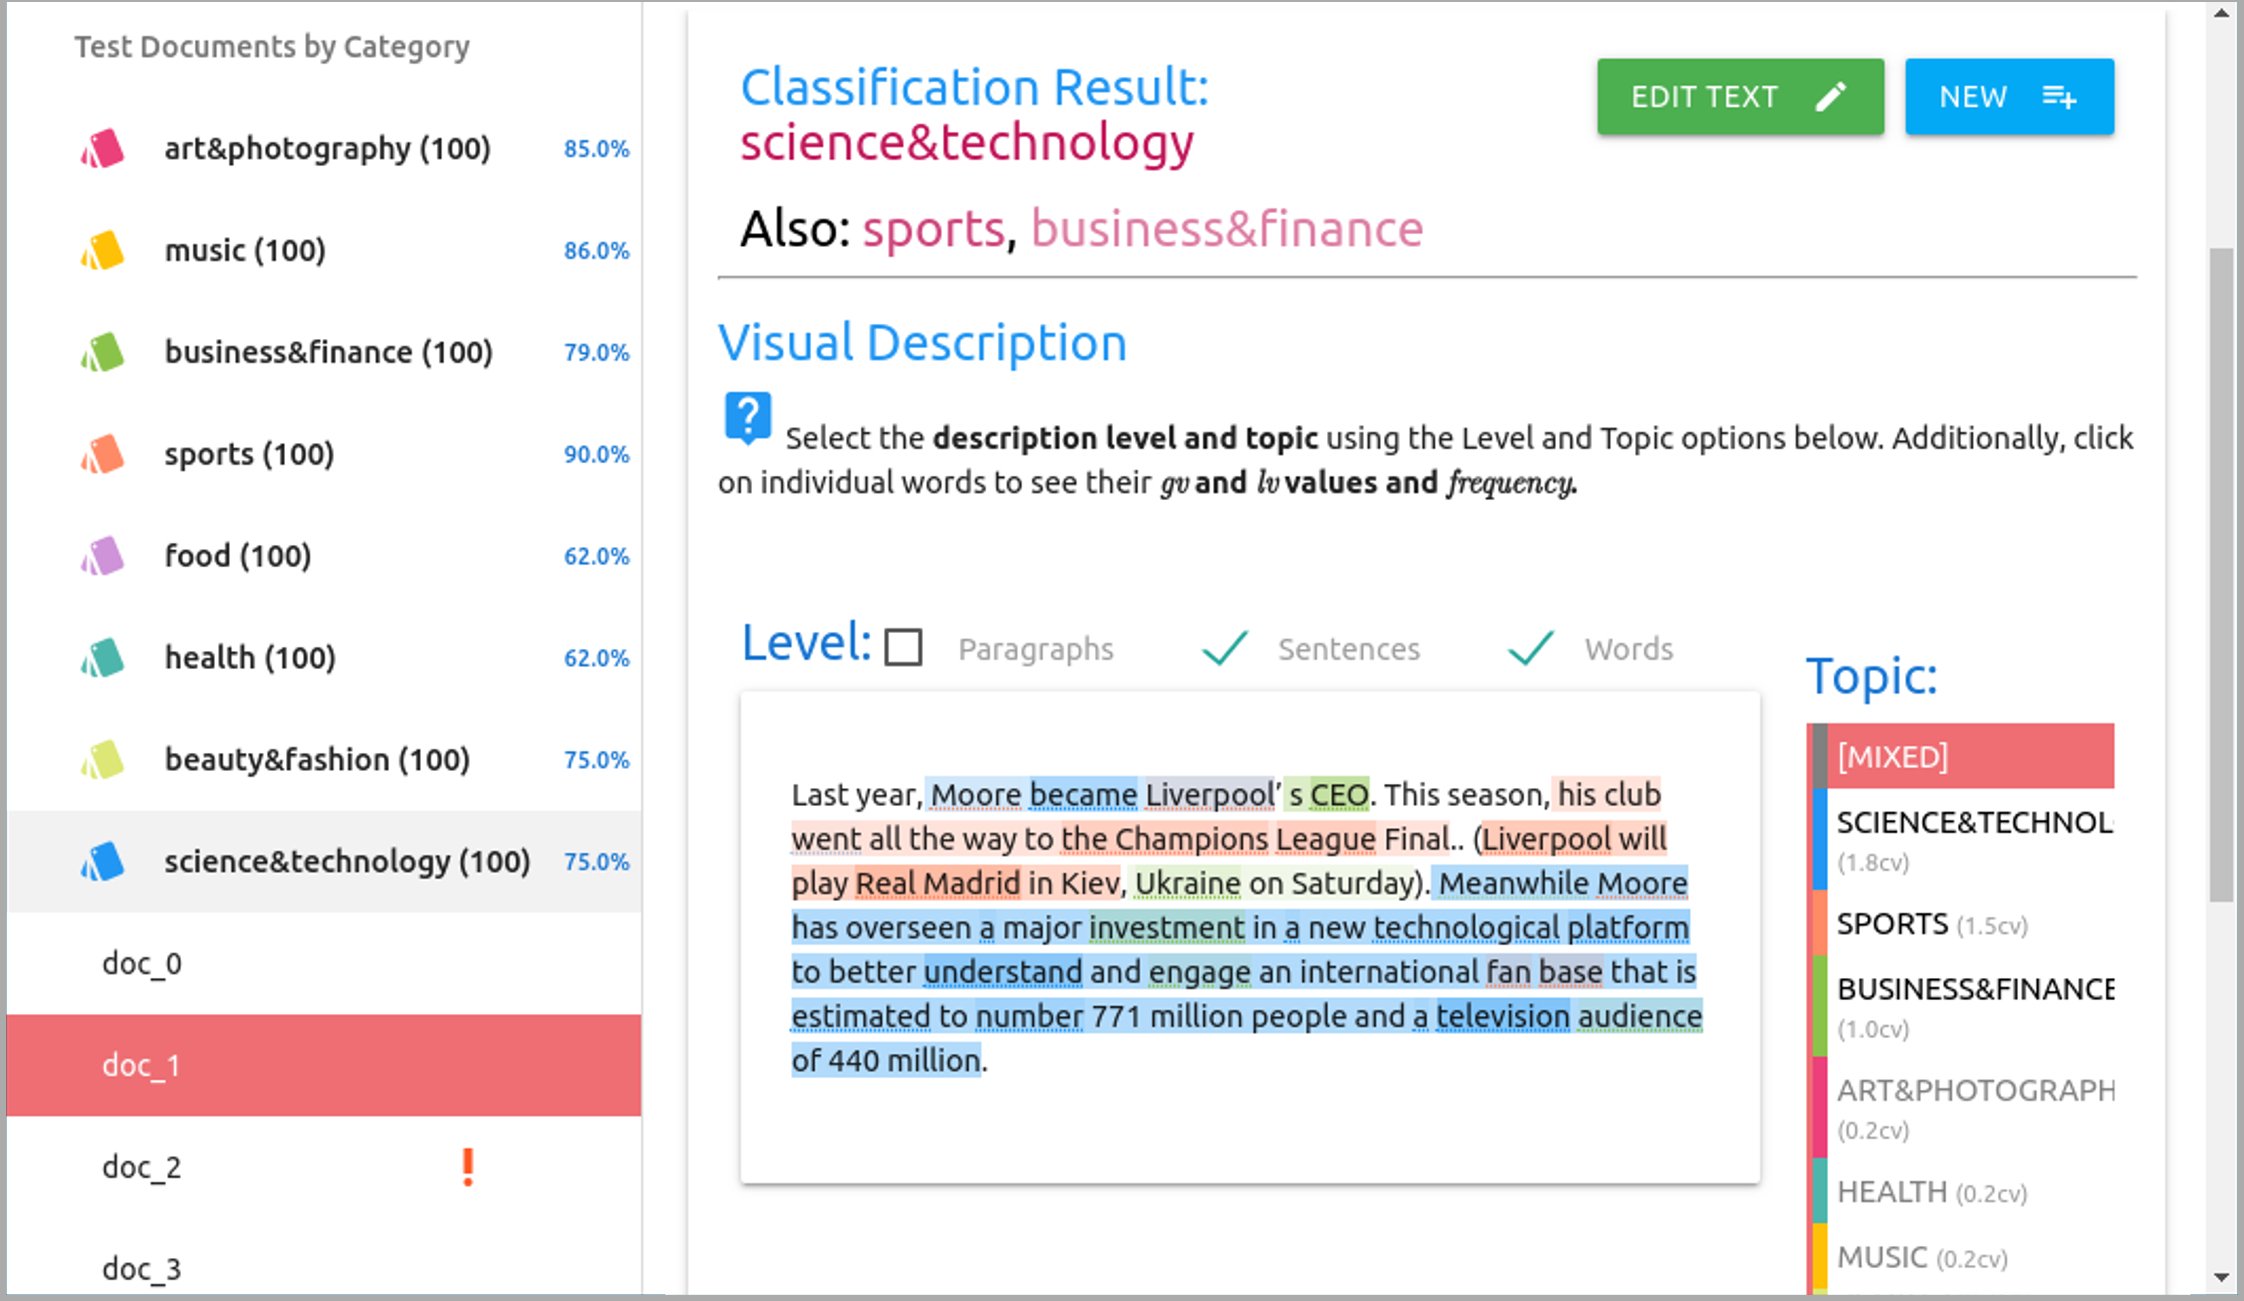
\includegraphics[width=\textwidth]{images/burdisso-fig1}
    \caption{
    Captura de pantalla de la herramienta ``Live Test''. En el panel izquierdo, se muestra la lista de documentos de prueba agrupados por clase, junto con el porcentaje de aciertos para cada una.
    Notar que el documento ``doc\_2'' está marcado con un signo de exclamación (!); esta marca indica que se lo clasificó de forma incorrecta, lo que facilita el análisis de errores.
    En este ejemplo, el usuario ha seleccionado el ``doc\_1'', el resultado de la clasificación se muestra en la parte superior.
    Además, el usuario ha seleccionado que la explicación visual sea dada a nivel de oración y de palabra en simultáneo.
    Por medio de esta explicación el usuario tal vez podría confirmar que el documento fue clasificado correctamente porque, efectivamente, el modelo ha aprendido a reconocer palabras importantes, como ser ``television'' para tecnología, ``Real Madrid'' para deportes o ``investment'' para negocios.
    Además, utilizando los distintos colores, el usuario podría notar que la primera oración pertenecía a varios temas, la segunda cambiaba el tema a deportes (naranja) y, finalmente, de ``Meanwhile'' en adelante, el tema se cambia principalmente a tecnología (azul), y un poco de negocios (verde) dado por las palabras ``investment'', ``engage'' y ``audience''.
    Finalmente, el usuario también podría editar el documento o crear uno nuevo utilizando los dos botones mostrados en la esquina superior derecha.}
    % Live Test screenshot. On the left side, the list of test documents grouped by category is shown along with the percentage of success.
    % Note the ``doc\_2'' document is marked with an exclamation mark (!); this mark indicates it was misclassified, which eases error analysis.
    % The user has selected the ``doc\_1,'' the ``classification result'' is shown above the visual description. 
    % In this figure, the user has chosen to display the visual explanation at sentence-and-word level, using mixed topics.
    % For instance, the user can confirm that, apparently, the model has learned to recognize important words and that it has correctly classified the document.
    % Also, by using the colors, the user could notice that the first sentence belonging to multiple topics, the second sentence shifted the topic to $sports$, and finally, from ``Meanwhile'' on, the topic is shifted to $technology$ (and a little bit of $business$ given by the words ``investment'' or ``engage'' colored in green).
    % Note that the user can also edit the document or even create new ones using the two buttons on the upper-right corner.}
    \label{fig:live_test}
\end{figure*}

La herramienta ``Live Test'' es una herramienta de visualización interactiva que le permite a los usuarios probar sus modelos de forma dinámica, en tiempo real.
% The ``Live Test'' tool is an interactive visualization tool that allows users to test his/her models ``on the fly.''
Esta herramienta se puede iniciar con una sola línea de código utilizando la clase ``Live\_Test'', como se mostrará con un ejemplo en la \autoref{sec:eg-2}.
Una vez iniciada, la herramienta proporciona una interfaz de usuario, como la mostrada en la \autoref{fig:live_test}, mediante la cual los usuarios pueden probar su modelo de forma activa utilizando ya sea los documentos del conjunto de prueba o simplemente escribiendo los suyos.
El objetivo principal de esta herramienta es permitirle a los usuarios analizar y comprender lo que efectivamente están aprendiendo sus modelos, por medio de explicaciones visuales similares a las mostradas al final del \autoref{cap:ss3} y \autoref{cap:tss3}, a diferentes niveles, n-gramas de palabras, oraciones y/o párrafos.
Esta herramienta es la que se utilizó para desarrollar las demos disponibles en línea mencionadas en los capítulos anteriores.\footnote{Disponibles en  \url{http://tworld.io/ss3}}
% This tool can be launched with a single line of python code using the $Server$ class (see \autoref{sec:eg-2} for an example).
% The tool provides a user interface (a screenshot is shown in \autoref{fig:live_test}) by which users can manually and actively test their model using either the documents in the test set or just typing  their own. 
% The tool also allows researchers to analyze and understand what their models are learning by providing an interactive and visual explanation of the classification process at three different levels (word n-grams, sentences, and paragraphs). 
% We recommend trying out the ``Topic Categorization'' or the ``Sentiment Analysis on Movie Reviews'' online live demo available at \href{http://tworld.io/ss3}{\url{http://tworld.io/ss3}}.

Por otro lado, la herramienta ``PySS3 Command-Line'' es una herramienta de línea de comandos interactiva, la cual se inicia desde la línea de comandos del sistema operativo utilizando el comando ``pyss3'', el cual se agrega automáticamente al sistema junto con la instalación del paquete.
Esta herramienta le permite a los usuarios implementar modelos SS3 e interactuar con ellos sin tener que programarlos utilizando Python, sino a través de la utilización de comandos especiales para cada etapa del proceso de desarrollo del modelo. Probablemente una de las características más importantes de esta herramienta es la capacidad de registrar, automática y permanentemente, el historial de cada evaluación que el usuario ha realizado sobre el modelo ---por ejemplo, utilizando validaciones cruzadas o búsquedas en grilla. Luego, los usuarios pueden utilizar este historial de evaluación para visualizar el rendimiento de sus modelos en términos de los distintos valores de los hiperparámetros, por medio del comando ``plot evaluations'' ---como se ilustrará en la \autoref{sec:eg-3}, estas mismas características también están disponibles a través de la clase $pyss3.util.Evaluation$.
% The ``PySS3 Command-Line'' is an interactive command-line tool that  can be started from the operating-system command prompt using the ``pyss3'' command (automatically added to the system when installing the package).
% This tool allows users to deploy SS3 models and interact with them through special commands for every stage of the machine learning pipeline (such as model selection, training, or testing). Probably one of its most important features is the ability to automatically (and permanently) record the history of every evaluation that the user has performed (such as tests, k-fold cross-validations, or grid searches). Users can then use this evaluation history to visualize their models' performance in terms of the hyperparameters' values though the ``plot evaluations'' command. As will be illustrated in \autoref{sec:eg-3}, the same features are also available through the $pyss3.util.Evaluation$ class.

\section{Ejemplos Ilustrativos}
\label{sec:examples}

En esta última sección, se presentan tres simples ejemplos ilustrativos que sirven para mostrar cómo se utiliza efectivamente el paquete en la práctica.
Como se menciona en la documentación del paquete, PySS3 proporciona dos tipos distintos de flujos de trabajo principales.
En el flujo de trabajo clásico, el usuario, como de costumbre, importa las clases y funciones necesarias del paquete, y luego escribe un programa Python para entrenar y probar los clasificadores. En el segundo flujo de trabajo, todo el proceso se realiza por medio de la herramienta ``PySS3 Command-Line'', sin tener que utilizar Python.
En esta sección no mostraremos ejemplos de este último, 
% In this section, we will introduce three simple illustrative examples.
% PySS3 provides two main types of workflow.
% In the classic workflow, the user, as usual, imports the needed classes and functions from the package and then writes a python script to train and test the classifiers. In the ``command-line'' workflow, the whole machine learning pipeline is done using only the ``PySS3 Command-Line'' tool, without coding in Python.
% Due to space limitations, we will not show examples for the latter here.
sin embargo, para ver ejemplos completos para ambos flujos de trabajo, se recomienda realizar alguno de los tutoriales disponibles en la documentación.\footnote{\url{https://pyss3.rtfd.io/en/latest/user_guide/getting-started.html\#tutorials}}
% However, for full working examples using both workflows, please refer to the tutorials in the documentation (\href{https://pyss3.rtfd.io/en/latest/user_guide/getting-started.html#tutorials}{\url{https://pyss3.rtfd.io/en/latest/user_guide/getting-started.html\#tutorials}})
Además, para los lectores interesados en probar el paquete en línea, sin tener que instalar nada en sus sistemas, los tutoriales también se encuentran disponibles en formato de Jupyter Notebooks, las cuales se pueden ejecutar en línea por medio del servicio \emph{MyBinder}.\footnote{Por medio del siguiente enlace: \url{https://mybinder.org/v2/gh/sergioburdisso/pyss3/master?filepath=examples}}
% Additionally, readers interested in trying PySS3 out ``right away'', we have created Jupyter Notebooks for the tutorials, which can be executed online using \emph{MyBinder} (\href{https://mybinder.org/v2/gh/sergioburdisso/pyss3/master?filepath=examples}{\url{https://mybinder.org/v2/gh/sergioburdisso/pyss3/master?filepath=examples}}).

\

Los siguientes ejemplos asumen que el usuario ya ha cargado los documentos de entrenamiento y prueba, y sus correspondientes etiquetas de clase, respectivamente, en las listas $x\_train$, $y\_train$, $x\_test$, $y\_test$, como es usual. Esto se podría llegar a hacer, por ejemplo, con $pyss3$ por medio de la clase ``Dataset'' del submódulo $pyss3.util$, de la siguiente manera:
% In the following examples, we will assume the user has already loaded the training and test documents and category labels, as usual, in the $x\_train$, $y\_train$, $x\_test$, $y\_test$ lists, respectively. For instance, this could be done using the $Dataset$ class from the $pyss3.util$ submodule, as follows:

\begin{minted}[
% frame=lines,
framesep=2mm,
baselinestretch=1.2,
bgcolor=lightgray,
fontsize=\footnotesize,
% linenos
]{python}
from pyss3.util import Dataset

x_train, y_train = Dataset.load_from_files("path/to/train")
x_test, y_test = Dataset.load_from_files("path/to/test")
\end{minted}


\subsection{Entrenamiento y Prueba}
\label{sec:eg-1}

En este pequeño ejemplo se muestra cómo, con unas pocas líneas y de forma similar a con los modelos de \emph{scikit-learn}, se puede entrenar y probar un modelo SS3 utilizando los valores predeterminados.
% This simple example shows how to train and test an SS3 model using default values.

\begin{minted}[
% frame=lines,
framesep=2mm,
baselinestretch=1.2,
bgcolor=lightgray,
fontsize=\small,
% fontsize=\footnotesize,
% linenos
]{python}
from pyss3 import SS3

clf = SS3()
clf.fit(x_train, y_train)

y_pred = clf.predict(x_test)
print("Accuracy:", accuracy(y_pred, y_test))
\end{minted}

La última línea imprime el \emph{accuracy} obtenido ---se asume aquí que la función \emph{accuracy} ya existe, por ejemplo, habiendo sido previamente importada desde \emph{sklearn.metrics}.
Notar que, dado que SS3 ignora el concepto de ``documento'' por su naturaleza, a diferencia de con los modelos de \emph{scikit-learn}, aquí no es necesario crear la matriz documento-término ---en su lugar, simplemente se utiliza directamente el texto (preprocesado) de los documentos de $x\_train$ y $x\_test$, tanto para el entrenamiento como para la prueba, respectivamente.
% The last line prints the obtained accuracy, we are assuming here that this $accuracy$ function already exists (for instance, it was previously imported from $sklearn.metrics$).
% Note that since SS3 creates a language model for each category, we do not need to create a document-term matrix, we are simply using the raw $x\_train$ and $x\_test$ documents for training and test, respectively.


\subsection{Entrenamiento y Prueba Interactiva}
\label{sec:eg-2}

En este ejemplo, al igual que en el anterior, se entrena y prueba el modelo. Sin embargo, en lugar de simplemente usar $predict$ y $accuracy$ para medir el rendimiento del modelo, aquí se utiliza la herramienta ``Live Test'', mostrada anteriormente en la \autoref{fig:live_test}, para analizar y probar nuestro modelo de una forma visual e interactiva, del siguiente modo:
% This example is similar to the previous one. However, instead of simply using $predict$ and $accuracy$ to measure our model's performance, here we are using the ``Live Test'' tool to analyze and test our model visually.

\begin{minted}[
% frame=lines,
framesep=2mm,
baselinestretch=1.2,
bgcolor=lightgray,
fontsize=\small,
% linenos
]{python}
from pyss3 import SS3
from pyss3.server import Live_Test

clf = SS3()
clf.fit(x_train, y_train)

Live_Test.run(clf, x_test, y_test)
\end{minted}

Esta última sentencia será la encargada de ejecutar la herramienta ``Live Test'' localmente en el navegador web, utilizando el clasificador, los documentos, y las etiquetas del conjunto de prueba dados en los argumentos.


Alternativamente, también se podría utilizar la función $clf.extract\_insight()$ que, cuando se aplica a un documento, devuelve la lista de fragmentos de texto involucrados en la decisión de la clasificación, ordenados por valor de confianza. Por ejemplo, supongamos que queremos obtener el fragmento de texto, con el mayor valor de confianza, que SS3 utilizó para clasificar al documento mostrado en la \autoref{fig:live_test} como ``sports'', entonces se podría simplemente utilizar $clf.extract\_insight()$ del siguiente modo:
% Alternatively, we could also use the $clf.extract\_insight()$ function. When this function is applied to a document, it returns the list of text fragments involved in the classification decision, ordered by confidence value. For instance, suppose we need to obtain the text fragment with the highest confidence value that was used to classify the document shown in \autoref{fig:live_test} as ``sports,'' we could use $extract\_insight()$ as follows:

\begin{minted}[
% frame=lines,
framesep=2mm,
baselinestretch=1.2,
bgcolor=lightgray,
fontsize=\small,
% linenos
]{python}
# doc = el mismo documento que se muestra en la Figura 7.1
doc = "Last year, Moore became Liverpool's CEO. This season, ..."

fragments = clf.extract_insight(doc, "sports")

print(fragments[0])
\end{minted}

% Which will print the following (fragment, confidence value) pair:
Lo que imprimirá el siguiente par (fragmento, valor de confianza):

\begin{minted}[
% frame=lines,
framesep=2mm,
baselinestretch=1.2,
bgcolor=lightgray,
fontsize=\small,
breaklines
% linenos
]{python}
('to the Champions League Final. (Liverpool will play Real Madrid in Kiev, Ukraine on Saturday). Meanwhile Moore has',  0.97)
\end{minted}

Este par nos indica que el documento fue clasificado como ``sports'', principalmente, debido a que nuestro modelo encontró este fragmento como perteneciente a ``sports'' con un valor de confianza de $0.97$.\footnote{Se recomienda el tutorial ``\emph{getting the text fragments involved in the classification decision}'' para los lectores interesados en conocer más sobre esta funcionalidad, disponible en  \url{https://pyss3.rtfd.io/en/latest/tutorials/extract-insight.html}} 
% This pair indicates the document was classified as ``sports,'' mainly due to our model finding this fragment as belonging to ``sports'' with a confidence value of $0.97$. Finally, interested readers may refer to the ``getting the text fragments involved in the classification decision'' tutorial available online (\href{https://pyss3.rtfd.io/en/latest/tutorials/extract-insight.html}{\url{https://pyss3.rtfd.io/en/latest/tutorials/extract-insight.html}}).

\subsection{Optimización de Hiperparámetros}
\label{sec:eg-3}

\begin{figure*}[t!]
    \centering
    % \includegraphics[width=190mm]{images/evaluation_plot}
    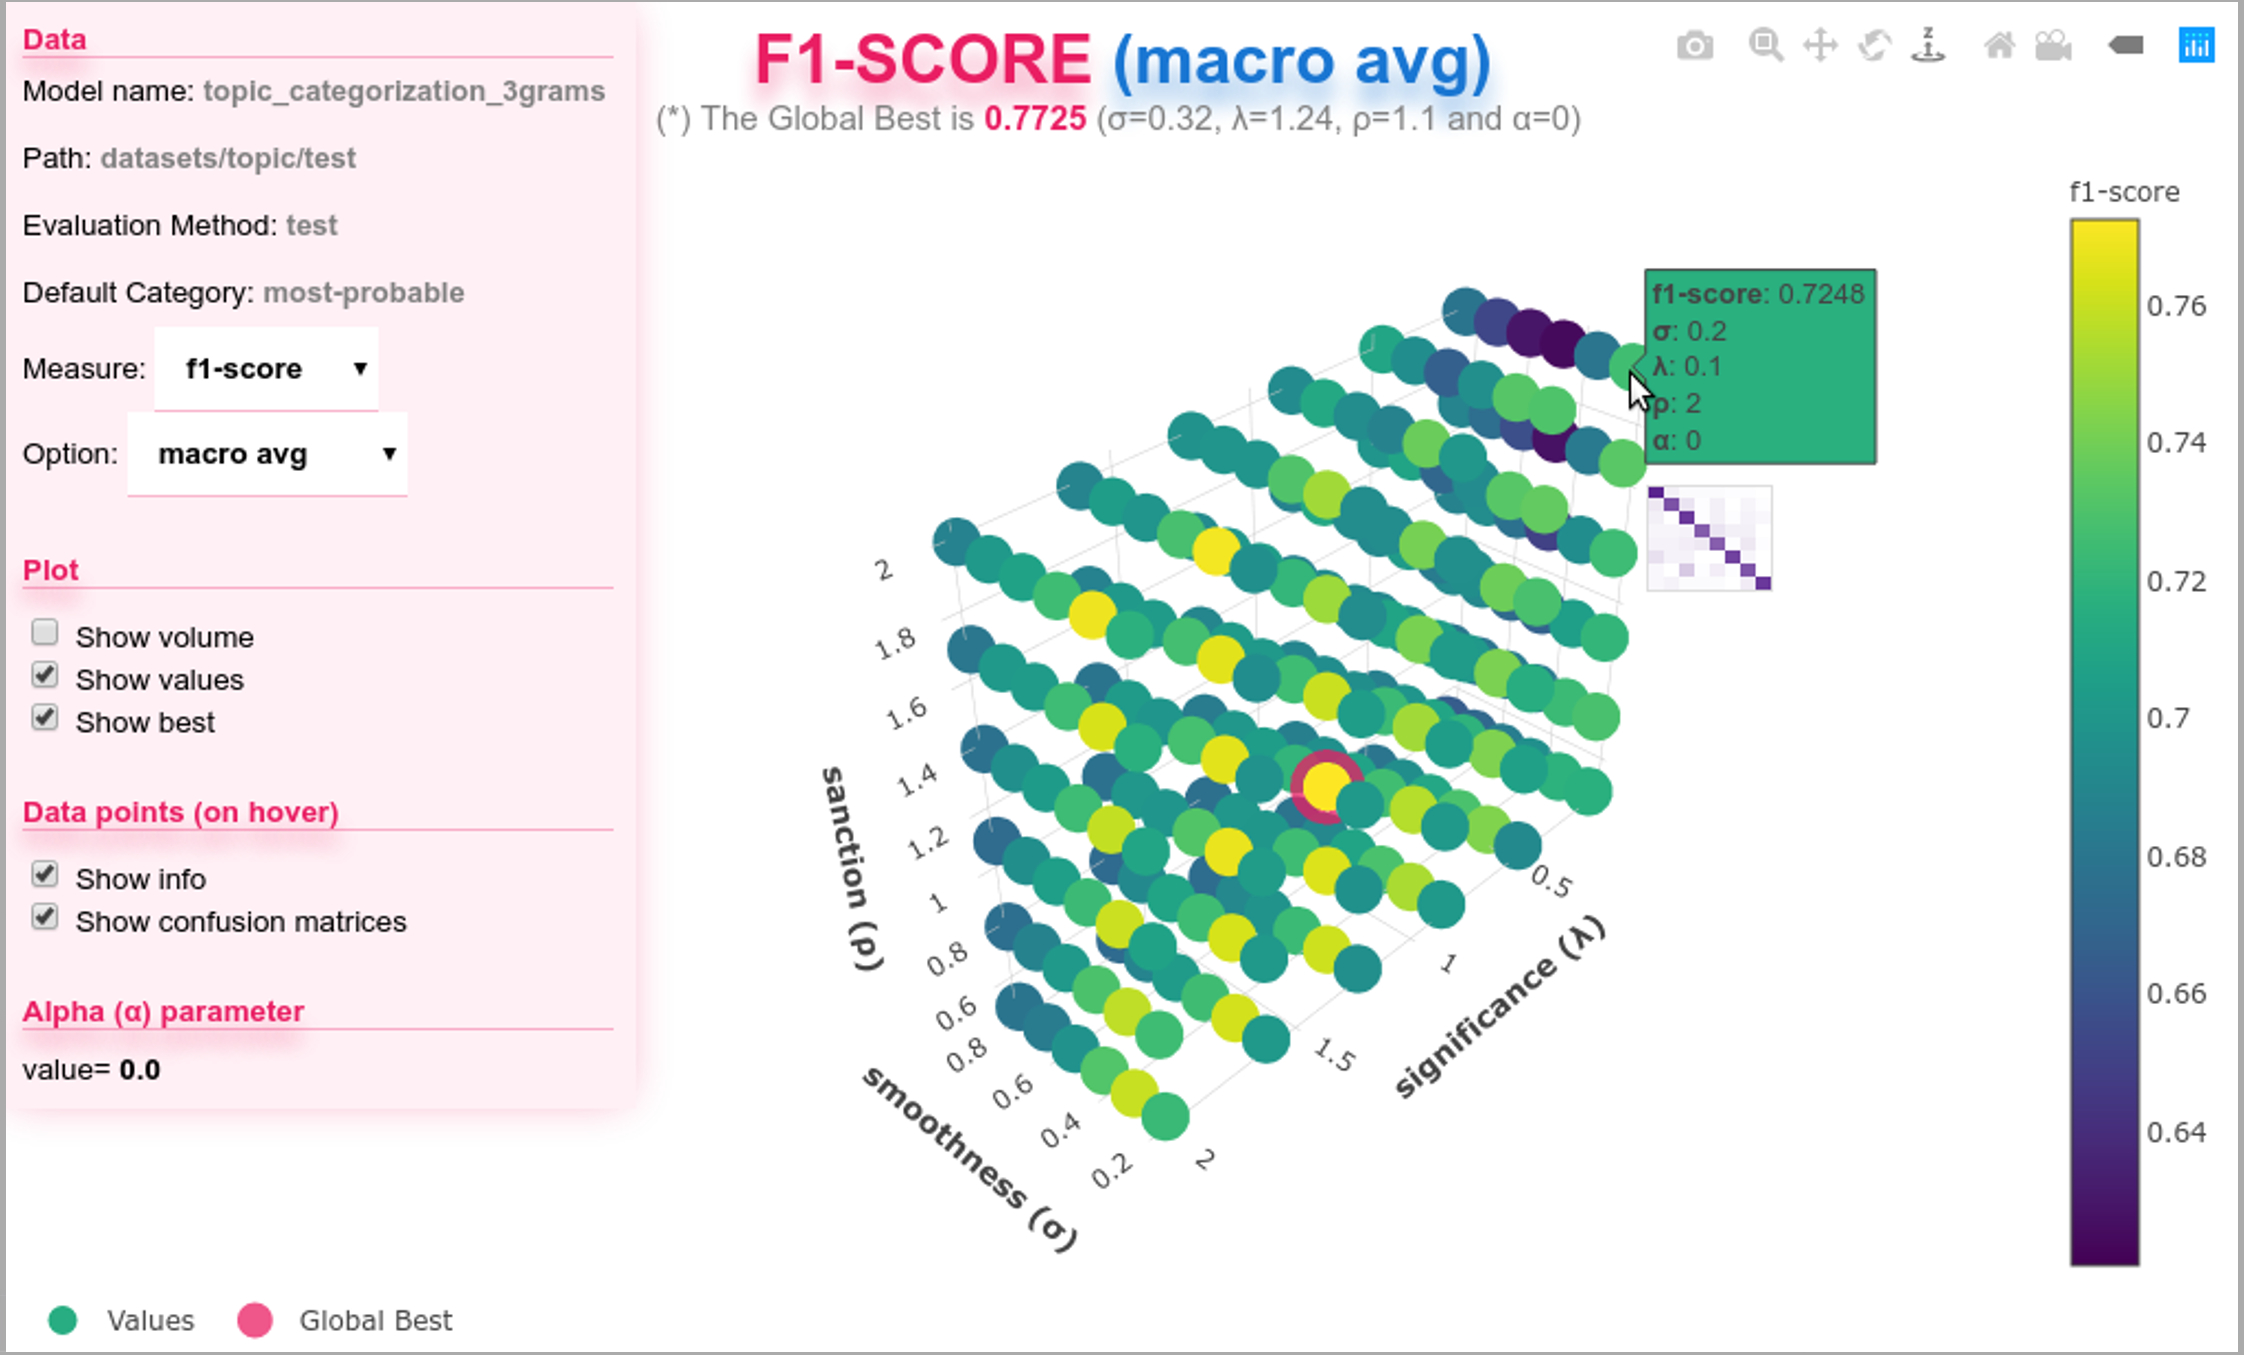
\includegraphics[width=\textwidth]{images/burdisso-fig2}
    \caption{Captura de pantalla del gráfico de evaluación 3D. Cada punto representa una evaluación o experimento realizado utilizando una combinación particular de valores de hiperparámetros. A su vez, estos puntos están coloreados proporcionalmente en relación al desempeño obtenido en esa evaluación. Además, en rosa se colorea el o los puntos que obtuvieron el mejor desempeño global. 
    El usuario puede seleccionar interactivamente la medida de evaluación que desee para medir el desempeño, cambiándola desde el panel de opciones mostrado a la izquierda.
    Además, como se muestra en esta figura, cuando el usuario mueve el cursor sobre un punto en particular, se muestra información relacionada con esa evaluación, incluida una versión simplificada de la matriz de confusión obtenida.}
    % \caption{Evaluation plot screenshot. Each data point represents an evaluation/experiment performed using a particular combination of hyperparameter values. Points are colored proportionally to the obtained performance. The performance measure can be interactively changed using the options panel in the upper-left corner. Additionally, points with the global best performance are marked in pink. As shown in this figure, when the user moves the cursor over a point, information related to that evaluation is displayed, including a small version of the obtained confusion matrix.}
    \label{fig:eval_plot}
\end{figure*}

Este último ejemplo muestra cómo, utilizando la clase ``Evaluation'', se pueden encontrar mejores valores de hiperparámetros para nuestro modelo. En particular, realizaremos la optimización de hiperparámetros por medio de una búsqueda en grilla, utilizando el método $grid\_search$ de la siguiente manera:
% This example shows how we could use the ``Evaluation'' class to find better hyperparameter values for the model trained in the previous example. Namely, we will perform hyperparameter optimization using the \emph{grid search} method, as follows:

\begin{minted}[
% frame=lines,
framesep=2mm,
baselinestretch=1.2,
bgcolor=lightgray,
fontsize=\small,
% linenos
]{python}
from pyss3.util import Evaluation

best_s, best_l, best_p, _ = Evaluation.grid_search(
    clf,
    x_test, y_test,
    s=[0.2, 0.32, 0.44, 0.56, 0.68, 0.8],
    l=[0.1, 0.48, 0.86, 1.24, 1.62, 2],
    p=[0.5, 0.8, 1.1, 1.4, 1.7, 2]
)
\end{minted}

Notar que en PySS3, los hiperparámetros $\sigma$, $\lambda$ y $\rho$  son referidos con las letras ``s'', ``l'' y ``p'', respectivamente.
% Note that in PySS3, the $\sigma$, $\lambda$, and $\rho$ hyperparameters are referenced using the ``s,'' ``l,'' and ``p'' letters, respectively.
Por lo tanto, en esta búsqueda en grilla, $\sigma$ tomará distintos valores diferentes entre $0.2$ y $0.8$, $\lambda$ entre $0.1$ y $2$, y $\rho$ entre $0.5$ y $2$.
% Thus, in this grid search, $\sigma$ will take six different values between $0.2$ and $0.8$, $\lambda$ between $0.1$ and $2$, and $\rho$ between $0.5$ and $2$.
Una vez finalizada la búsqueda, esta función devolverá los mejores valores obtenidos para los tres hiperparámetros, asignándolos respectivamente a $best\_s$, $best\_l$ y $best\_p$.
% Also note that once the grid search is over, the function will return the best hyperparameter values and store them in $b\_s$, $b\_l$, and $b\_p$, respectively.

Luego de realizar la búsqueda en grilla, para poder realizar un mejor análisis del desempeño obtenido en la búsqueda, podríamos utilizar la función $plot()$ para visualizar los resultados con un gráfico tridimensional, de la siguiente manera:
% After performing the grid search, we could also use the $plot()$ function to visualize our results, as follows:

\begin{minted}[
% frame=lines,
framesep=2mm,
baselinestretch=1.2,
bgcolor=lightgray,
fontsize=\small,
% linenos
]{python}
Evaluation.plot()
\end{minted}

Esta función creará en el directorio actual un archivo HTML portátil que contiene un gráfico 3D interactivo, y luego lo abrirá en el navegador web del usuario.
% This function will first save, in the current directory, a single and portable HTML file containing an interactive 3D plot. Then, it will open it up in the web browser.
Por ejemplo, en la \autoref{fig:eval_plot} se muestra una captura de pantalla de este gráfico 3D, en el que podemos ver que los mejores valores de hiperparámetros para esta búsqueda fueron $\sigma=0.32$, $\lambda=1.24$ y $\rho=1.1$.
Finalmente, utilizando la función $clf.set\_hyperparameters()$ podríamos actualizar los hiperparámetros de nuestro modelo con los mejores valores obtenidos, de la siguiente manera:
% For instance, a screenshot of this 3D plot is shown in \autoref{fig:eval_plot}, \footnote{More info available in the documentation (\href{https://pyss3.rtfd.io/en/latest/user_guide/visualizations.html\#evaluation-plot}{\url{https://pyss3.rtfd.io/en/latest/user_guide/visualizations.html\#evaluation-plot}}).} 
% in which we can see that the best hyperparameter values for this search were $\sigma=0.32$, $\lambda=1.24$, and $\rho=1.1$. Finally, using the obtained best values, we could update the hyperparameter values of our already trained model using the $clf.set\_hyperparameters()$ function, as follows:

\begin{minted}[
% frame=lines,
framesep=2mm,
baselinestretch=1.2,
bgcolor=lightgray,
fontsize=\small,
% linenos
]{python}
clf.set_hyperparameters(s=best_s, l=best_l, p=best_p)
\end{minted}

Alternativamente, también podríamos crear y entrenar un nuevo modelo desde cero utilizando manualmente los mejores valores obtenidos:
% Alternatively, we could also create and train a new model using the obtained best values:

\begin{minted}[
% frame=lines,
framesep=2mm,
baselinestretch=1.2,
bgcolor=lightgray,
fontsize=\small,
% linenos
]{python}
clf = SS3(s=0.32, l=1.24, p=1.1)
clf.fit(x_train, y_train)
\end{minted}

\begin{figure}[t!]
    \centering
    % 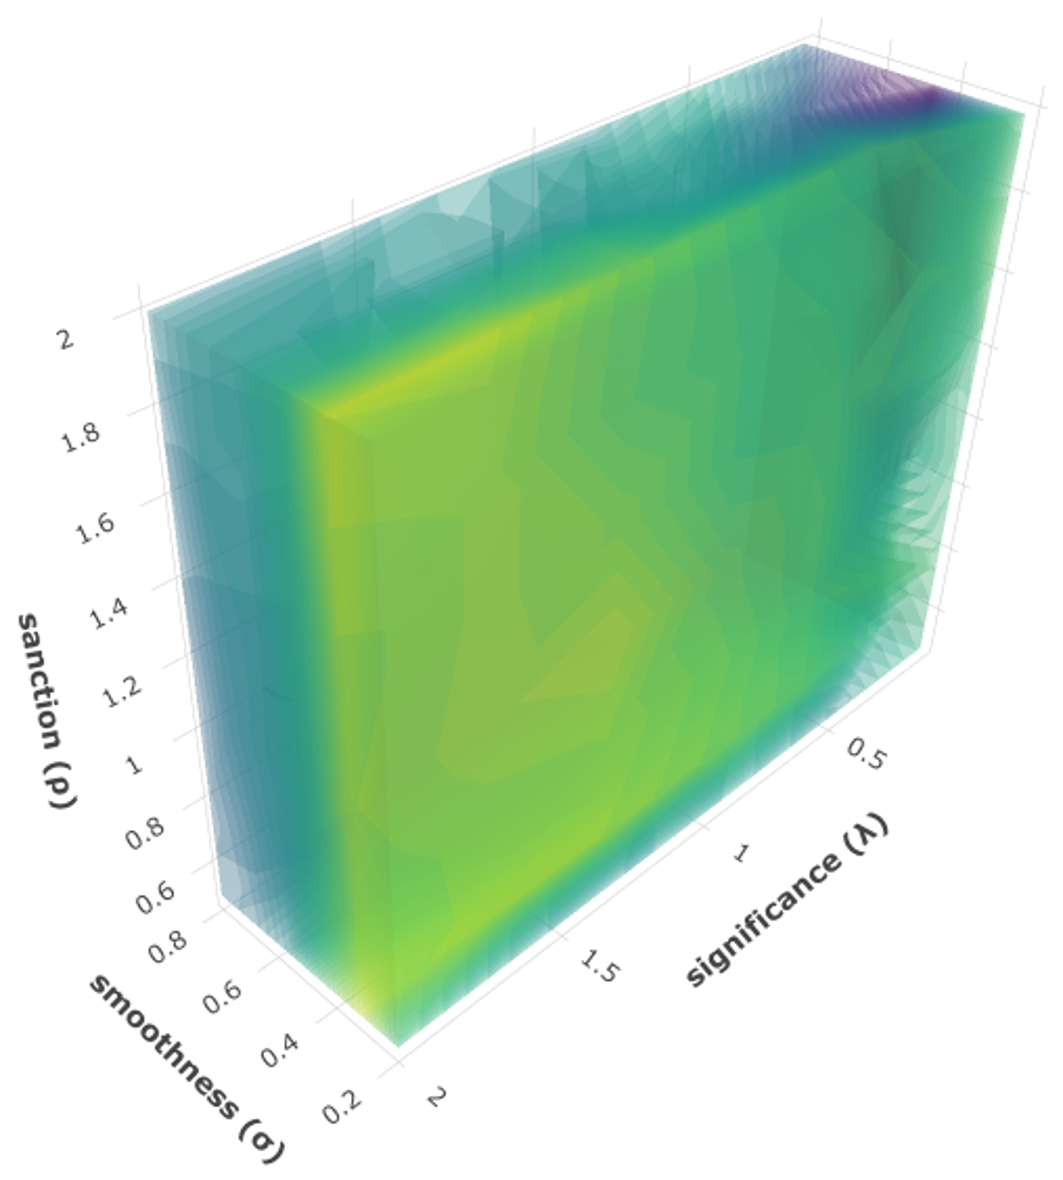
\includegraphics[width=\linewidth]{images/burdisso-fig3}
    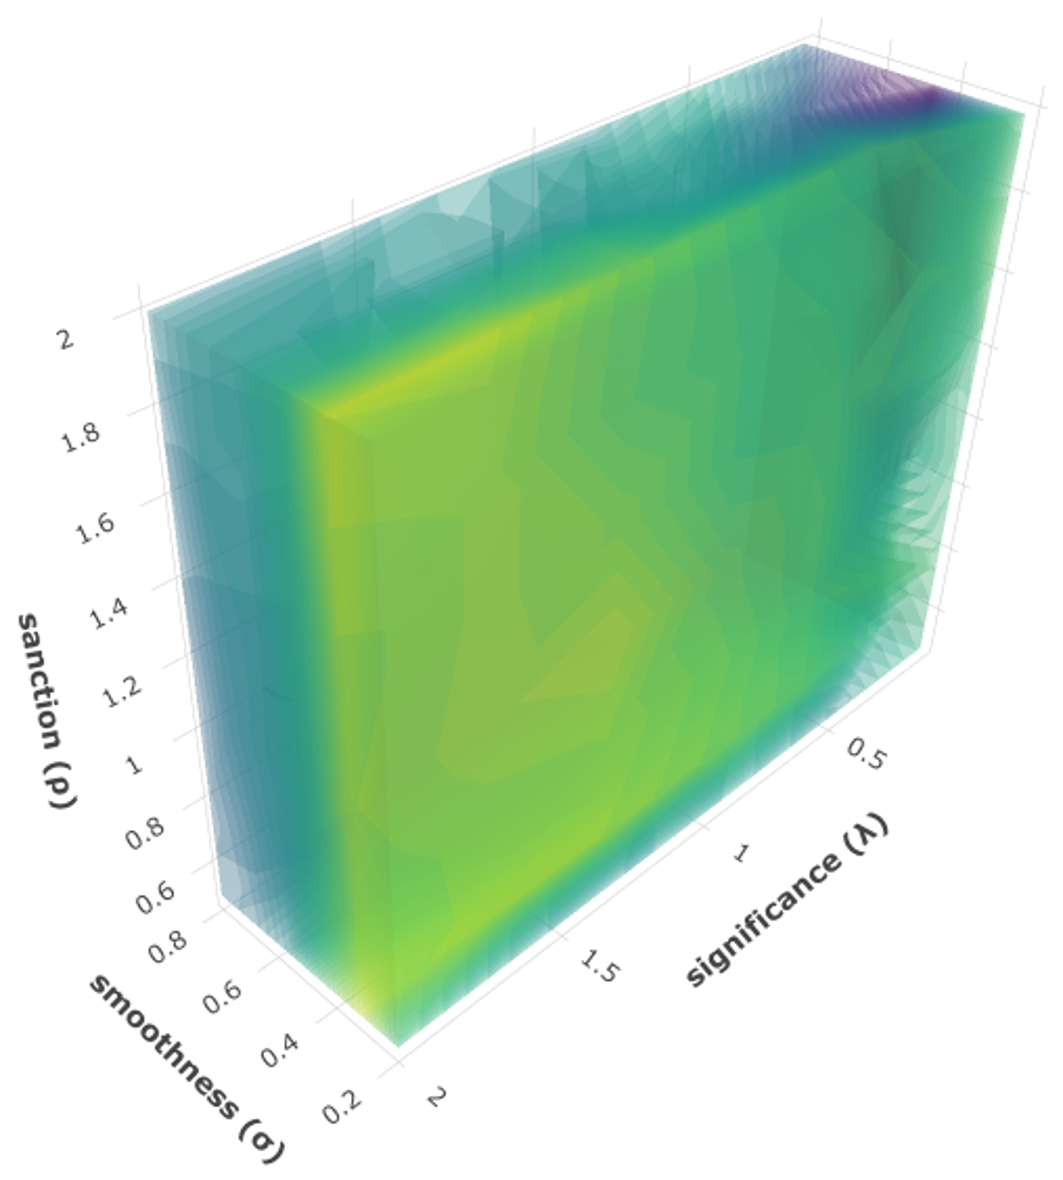
\includegraphics[width=90mm]{images/burdisso-fig3}
    \caption{Gráfico de evaluaciones con la opción ``show volume'' (mostrar volumen) habilitada. Al habilitar esta opción, ahora podemos observar más claramente que el hiperparámetro \emph{sanction} ($\rho$) no parece afectar el rendimiento. Por el contrario, el rendimiento parece aumentar a medida que aumenta el valor de \emph{significance} ($\lambda$) y parece disminuir a medida que el hiperparámetro \emph{smoothness} ($\sigma$) se aleja de $0.35$.}
    % \caption{Evaluation plot with ``show volume'' option enabled.  With this option enabled, we can now more clearly see that the \emph{sanction} ($\rho$) hyperparameter does not seem to impact performance. In contrast, the performance seems to increase as the \emph{significance} ($\lambda$) value increases and seems to drop as the \emph{smoothness} ($\sigma$) hyperparameter moves away from $0.35$.}
    \label{fig:eval_plot_volume}
\end{figure}

Notar que, además de utilizar el gráfico de evaluación 3D para obtener los mejores valores, los usuarios pueden utilizarlo para analizar, y comprender mejor, la relación entre los hiperparámetros y el rendimiento del clasificador dentro del problema particular abordado.
Por ejemplo, si el usuario habilita la opción ``show volume'' desde el panel de opciones, el gráfico se convertirá en una estructura sólida que nos facilitará  realizar este tipo de análisis, como se muestra en la \autoref{fig:eval_plot_volume}. Otra característica positiva de la función $Evaluation.plot()$ es que le permitirá a los investigadores compartir sus gráficos, por ejemplo en sus publicaciones, por medio de los archivos HTML portables generados localmente ---lo que aumentaría la transparencia de las experimentaciones.\footnote{Por ejemplo, hemos subido el archivo HTML generado para el ejemplo mostrado en la \autoref{fig:eval_plot} en línea para que los lectores interesados pueden interactuar con él: \url{https://pyss3.rtfd.io/en/latest/_static/eval_plot.html}}
% Note that, in addition to using the 3D evaluation plot to obtain the best values, users can use it to analyze (and better understand) the relationship between hyperparameters and performance in the particular problem being addressed. 
% For instance, if the ``show volume'' option is enabled from the options panel, the plot will turn into the plot shown in \autoref{fig:eval_plot_volume}. It is worth mentioning that researchers could share these portable files with the 3D plots in their papers, which would increase experimentation transparency. For instance, we have uploaded the file generated for \autoref{fig:eval_plot} online for readers to interact with it (\href{https://pyss3.rtfd.io/en/latest/_static/eval_plot.html}{\url{https://pyss3.rtfd.io/en/latest/_static/eval_plot.html}}).
%\footnote{It is worth mentioning that researchers could share these 3D model evaluation's portable files in their papers, which would increase experimentation transparency. For instance, we have uploaded the file used for the evaluation shown in \autoref{fig:eval_plot} for readers to interact with it: \href{https://pyss3.rtfd.io/en/latest/_static/eval_plot.html}{\url{https://pyss3.rtfd.io/en/latest/_static/eval_plot.html}}}

\section{Observaciones Finales}

En este capítulo hemos introducido brevemente a PySS3, un paquete de Python de código abierto que permite utilizar fácilmente el modelo de clasificación de texto desarrollado como producto de este trabajo de investigación. Además, este paquete incluye una serie de herramientas de visualización útiles que ayudan a comprender mejor lo que el modelo está realmente aprendiendo.
Este software podría ser especialmente útil para investigadores, profesionales o usuarios en general, interesados en implementar modelos más transparentes, y por lo tanto más confiables, para tareas de clasificación de texto.
Finalmente, esperamos continuar el avance y la mejora de PySS3 a través de la ayuda directa o indirecta de todos aquellos que estén interesados y quieran formar parte de este proyecto de código abierto.
% We have briefly introduced PySS3, an open-source Python package that implements a novel machine learning model for text classification that comes with useful visualization tools.
% This software could be especially useful for researchers and practitioners interested in deploying explainable and more reliable models for text classification.
% Finally, we hope to continue the advancement and improvement of PySS3 through the direct or indirect help of those in the mathematical and computer science disciplines who want to be part of this open-source project.
\hfill$\square$